%--------------------------------------------------------------------
% 4 Implementación – SEPA Request‑to‑Pay Prototype (Clase `article`)
%--------------------------------------------------------------------
\chapter{Implementación}
\label{sec:implementacion}

Este apartado traduce los principios definidos en el Diseño (Secc.~\ref{sec:diseno}) a código ejecutable. Cada subsección muestra la correspondencia entre los artefactos lógicos y su concreción en Python\,/\,JavaScript, de modo que se pueda verificar cómo se satisfacen los requisitos \textbf{RF} y \textbf{RNF} enumerados anteriormente.

%---------------------------------------------------------------
% 4.1 Visión general de la arquitectura y organización del código
%---------------------------------------------------------------
\section{Visión general de la arquitectura y organización del código}
\label{sec:impl-vision}

\noindent
La implementación del prototipo para simular un proveedor del esquema SRTP requiere una arquitectura robusta y una organización del código que garanticen la claridad, la mantenibilidad y la alineación con los requisitos establecidos en los capítulos anteriores. Este apartado ofrece una descripción detallada de la arquitectura general del sistema, explicando cómo se han estructurado sus componentes y cómo estos interactúan para cumplir con los objetivos del proyecto. Asimismo, se presenta la organización del código fuente, incluyendo la estructura de directorios, para ilustrar cómo se ha traducido el diseño conceptual del capítulo 3 en una implementación práctica. Esta sección no solo busca documentar las decisiones técnicas tomadas, sino también demostrar cómo el sistema aborda las limitaciones del SDD identificadas en la sección \ref{subsec:Motivacion}, como la necesidad de procesos más ágiles y en tiempo real.

La arquitectura adoptada se fundamenta en principios de modularidad, escalabilidad y separación de preocupaciones, lo que permite que cada parte del sistema tenga un propósito claro y que las interacciones entre componentes sean eficientes. A continuación, se describen los elementos clave de la arquitectura general, seguidos por una explicación de la organización del código y su estructura de directorios, acompañada de ejemplos concretos que refuerzan la conexión entre el diseño y la implementación.

\subsection{Componentes del servidor}
\label{subsec:componentes-del.serv}
\begin{itemize}
    \item \textbf{Capa de persistencia}: Esta capa se encarga de gestionar los datos del sistema utilizando un enfoque basado en modelos ORM (Object-Relational Mapping). Los modelos definidos aquí, como la entidad \texttt{RTP} que representa una solicitud de pago, están alineados con el diseño de la base de datos descrito en la sección \ref{subsec:diseno_datos}. La persistencia asegura que la información se almacene de forma estructurada y sea accesible para las operaciones del SRTP.
    
    \item \textbf{Capa de servicios de negocio}: Aquí reside la lógica central del prototipo, implementando las transiciones de estado del flujo SRTP (creación, validación, enrutamiento y decisión). Cada servicio está diseñado como un módulo independiente que encapsula las reglas de negocio, garantizando que las operaciones cumplan con los requisitos funcionales y no funcionales establecidos en el capítulo \ref{sec:diseno}.
    
    \item \textbf{Capa de interfaz pública}: Expone las funcionalidades del sistema mediante una API REST y un sistema de comunicación en tiempo real basado en WebSockets. La API REST ofrece endpoints bien definidos para operaciones síncronas, mientras que los WebSockets permiten notificaciones instantáneas a los actores, abordando directamente las ineficiencias de los ciclos de cobro del SDD mencionadas en la sección \ref{subsec:ineficiencias}.
\end{itemize}

\paragraph{Cliente}

El cliente es una aplicación web desarrollada con Vue.js, seleccionada por su capacidad para crear interfaces reactivas y dinámicas. Esta aplicación permite a los usuarios visualizar y gestionar solicitudes RTP, desde la creación por parte del beneficiario hasta la aceptación o rechazo por el pagador. La comunicación con el servidor se realiza a través de la API REST para operaciones como la creación de solicitudes, y mediante WebSockets para actualizaciones en tiempo real, como cambios de estado.

\paragraph{Interacción entre componentes}

La interacción entre el cliente y el servidor es un aspecto crítico del sistema. Por ejemplo, cuando un beneficiario crea una solicitud RTP, el cliente envía una petición a través de un endpoint REST al servidor, que procesa la solicitud en la capa de servicios y la almacena en la capa de persistencia. Una vez procesada, el servidor notifica a los actores relevantes mediante WebSockets, actualizando la interfaz del cliente en tiempo real. Este flujo refleja las decisiones de diseño de la sección \ref{subsec:diseno_requisitos}, donde se priorizó la agilidad y la inmediatez en las operaciones.


%---------------------------------------------------------------
\subsection{Estructura de directorios}
%---------------------------------------------------------------
\label{sec:impl-vision-tree}

La organización del código fuente ha sido diseñada para reflejar la arquitectura en capas del sistema y facilitar tanto el desarrollo como el mantenimiento del prototipo. La estructura de directorios de la figura \ref{fig:treeB} está pensada para que los desarrolladores puedan localizar rápidamente los componentes clave y comprender su propósito dentro del proyecto. A continuación, se detalla la estructura principal :

\vspace{.6em}
\paragraph*{Backend.}
Los ocho módulos Python se bastan para ofrecer una capa de servicios
coherente, auditable y sin dependencias circulares:

\begin{itemize}
  \item \texttt{app.py} actúa como \emph{bootstrap} del marco Flask;
        instancia la aplicación, registra los \emph{blueprints},
        inicializa la base de datos y arranca el \emph{Notification Hub}
        basado en Socket.IO, de modo que HTTP y WebSocket
        comparten proceso y puerto.
  \item \texttt{config.py} encapsula los parámetros de despliegue
        y proporciona
        valores seguros por defecto para ejecutarse
        en entornos de desarrollo sin intervención manual.
  \item \texttt{ext\_socketio.py} mantiene una única instancia global
        de \texttt{SocketIO}; centraliza la creación de salas
        y la emisión de eventos para evitar duplicidades y facilitar
        un eventual cambio de motor de concurrencia.
  \item \texttt{models.py} define las entidades
        \emph{Actor}, \emph{RTP} y \emph{Log} con SQLAlchemy,
        garantizando la integridad referencial y sellando cada transición
        con un hash SHA-256 que permite auditar el histórico.
  \item \texttt{routes.py} expone los cinco endpoints REST
        que materializan la máquina de estados SRTP; cada manejador se
        limita a validar parámetros y delegar la lógica en los servicios.
  \item \texttt{routes\_actors.py} ofrece
        operaciones auxiliares—registro y consulta de actores—que,
        aun no formando parte del flujo SRTP, resultan imprescindibles
        para montar un entorno de pruebas auto-contenido.
  \item \texttt{services.py} orquesta la lógica de dominio:
        comprueba pre-condiciones, transforma el estado,
        persiste los cambios y publica las notificaciones correspondientes;
        de esta forma aísla los detalles del transporte (REST o WebSocket)
        y favorece las pruebas unitarias.
  \item \texttt{utils.py} y \texttt{utils\_roles.py} concentran
        utilidades transversales: la primera agrupa funciones de apoyo
        (p.\,ej.\  \texttt{cambiar\_estado\_rtp} o la validación de IBAN),
        mientras que la segunda implementa el decorador
        \texttt{@role\_required}, responsable de aplicar el control de
        acceso antes de ejecutar cada endpoint.
\end{itemize}

\paragraph*{Frontend.}
Los recursos estáticos se limitan a cinco archivos, suficientes para
construir una SPA ligera pero reactiva:

\begin{itemize}
  \item \texttt{index.html} sirve de punto de entrada.
        Además de la cabecera de navegación, contiene el
        contenedor \texttt{\textless{}div id="root"\textgreater{}} donde los
        módulos JavaScript inyectan las vistas solicitadas.
  \item \texttt{RTP.html} almacena la plantilla que representa el
        \emph{workflow} SRTP; se carga bajo demanda para evitar penalizar
        el \emph{time-to-first-paint}.
  \item \texttt{styles.css} define la paleta corporativa, el
        \emph{grid} de disposición y las transiciones que dotan de
        fluidez a los cambios de estado.
  \item \texttt{app.js} gestiona la autenticación,
        el enrutado de vistas
        y la apertura de la conexión WebSocket, mostrando indicadores de
        estado (conectado, reconectando, \dots) sin recargar la página.
  \item \texttt{RTP.js} implementa toda la lógica de cliente
        relacionada con las solicitudes: construcción de formularios,
        llamadas al API REST y actualización en tiempo real de la tabla
        de notificaciones cuando llegan los eventos \emph{push}.
\end{itemize}

\vspace{.2em}
\paragraph*{Síntesis y trazabilidad.}
Esta disposición jerárquica refleja en el código la arquitectura
conceptual del capítulo \ref{sec:diseno}: la capa de presentación
(\emph{frontend}) permanece aislada de la de negocio
(\emph{backend}); la única superficie de contacto es la API REST
y el canal WebSocket, ambos documentados y versionados.
Gracias a ello, cualquier sustitución—cambiar el
motor de base de datos, desplegar la SPA en un CDN o
servir las peticiones HTTP detrás de un WAF—puede acometerse
sin modificar las capas restantes, cumpliendo así los
RNF de portabilidad y mantenibilidad establecidos
para el prototipo.

\begin{figure}[htbp]
  \centering
  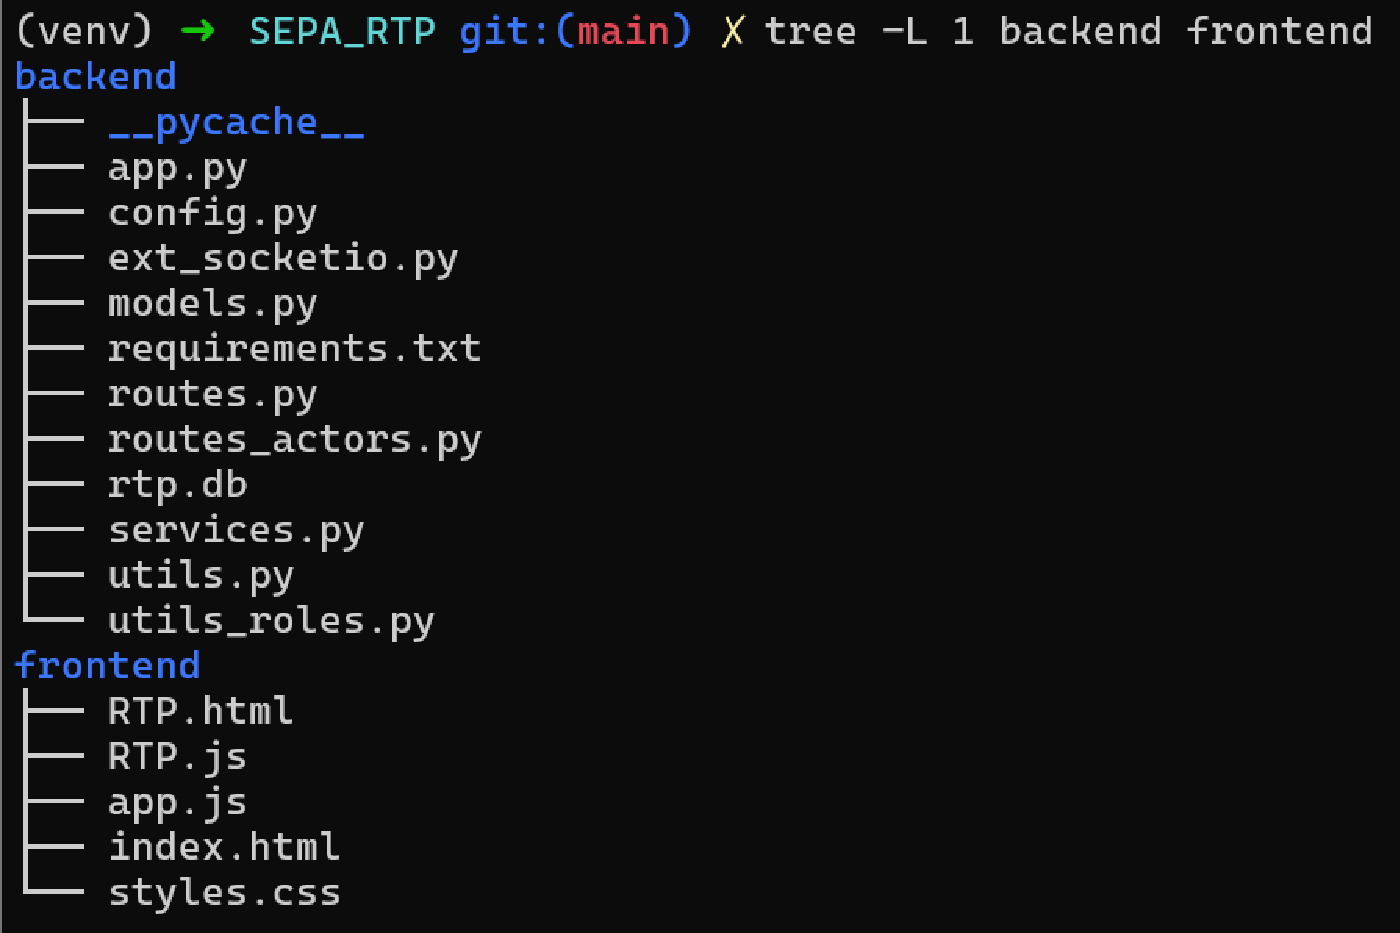
\includegraphics[width=.85\textwidth]{Imagenes/treeB.pdf}
  \caption{Estructura en árbol del directorio}
  \label{fig:treeB}
\end{figure}

Esta estructura promueve la modularidad y el aislamiento de responsabilidades. Por ejemplo, la separación entre \textbf{/models} y \textbf{/services} permite modificar la lógica de negocio sin afectar la persistencia.

%----------------------------------------------------------------
\subsection{Satisfacción de requisitos}
%----------------------------------------------------------------
Este subapartado tiene como objetivo demostrar de manera detallada cómo el prototipo implementado cumple con cada uno de los \textbf{requisitos funcionales (RF)} y \textbf{no funcionales (RNF)} establecidos en el capítulo \ref{sec:diseno}. Para cada requisito, se proporciona una explicación de su propósito dentro del flujo del esquema SRTP, se referencian los fragmentos de código que materializan la solución y se indica la ruta del archivo donde se aloja dicha lógica. Los fragmentos de código se han incluido en el \emph{Índice de listados} al final de la memoria para facilitar su localización y consulta.

La estructura de este apartado sigue el orden de los requisitos tal como fueron definidos, comenzando por los funcionales y continuando con los no funcionales. Cada explicación busca no solo describir la implementación, sino también conectar la solución técnica con las necesidades operativas del SRTP, destacando cómo el prototipo supera las limitaciones identificadas en el SEPA Direct Debit (SDD).

\begin{description}
%---------------------------------------------------------------
\item[RF-01 — Crear solicitud RTP]  
El primer requisito funcional, RF-01, se refiere a la capacidad del Beneficiario para crear una solicitud de pago RTP. Este paso es crucial en el flujo SRTP, ya que inicia el proceso de cobro y establece los parámetros de la transacción, como el IBAN del deudor, el importe y el concepto del pago. En el prototipo, esta funcionalidad se implementa mediante una petición HTTP POST al endpoint \texttt{/rtp}, que es gestionada por el backend para generar y persistir la entidad RTP en la base de datos.

La lógica principal de este requisito se encuentra en el archivo \texttt{services.py}, específicamente en la función encargada de crear la solicitud RTP. El fragmento de código correspondiente, mostrado en el Listado~\ref{lst:1}, realiza varias tareas clave: valida los datos de entrada, genera un hash idempotente para garantizar la unicidad de la solicitud y persiste la entidad en la base de datos con el estado inicial \textit{creado}. Este hash es fundamental para evitar duplicaciones y asegurar la integridad de las solicitudes, abordando así una de las ineficiencias operativas del SDD relacionadas con la gestión manual de mandatos.

El endpoint REST que expone esta funcionalidad al frontend se define en \texttt{routes.py}, y su implementación se presenta en el Listado~\ref{lst:2}. Este handler recibe la petición del cliente, delega la lógica de negocio al servicio correspondiente y devuelve una respuesta adecuada. Desde el lado del cliente, el archivo \texttt{RTP.js} contiene la rutina JavaScript que serializa los datos del formulario y envía la petición POST al backend, como se muestra en el Listado~\ref{lst:3}. Esta interacción entre el frontend y el backend asegura que el Beneficiario pueda crear solicitudes RTP de manera intuitiva y eficiente, cumpliendo con el requisito RF-01.

%---------------------------------------------------------------
\item[RF-02 — Validar y enrutar (PSP Beneficiary)]  
El requisito RF-02 abarca dos acciones críticas realizadas por el PSP del Beneficiario: la validación de la solicitud RTP y su posterior enrutamiento hacia el PSP del Pagador. La validación implica verificar la corrección sintáctica de los datos, como la validez de los IBAN y la coherencia del importe, mientras que el enrutamiento consiste en preparar la solicitud para su envío al siguiente actor en el flujo SRTP.

Para la validación, el prototipo utiliza un algoritmo para comprobar la validez de los IBAN, implementado en la función correspondiente del archivo \texttt{utils.py}, como se detalla en el Listado~\ref{lst:6}. Este paso es esencial para prevenir errores en las transacciones y garantizar la integridad de los datos antes de proceder con el enrutamiento.

Una vez validada la solicitud, los servicios definidos en \texttt{services.py} actualizan el estado de la entidad RTP a \textit{validado\_beneficiario} y posteriormente a \textit{enrutado}, notificando al PSP del Pagador sobre la nueva solicitud. Estos servicios se presentan en el Listado~\ref{lst:4}. Los controladores REST que exponen estas funcionalidades se encuentran en \texttt{routes.py}, específicamente en los endpoints dedicados a la validación y enrutamiento, como se muestra en el Listado~\ref{lst:5}. En el frontend, el archivo \texttt{RTP.js} incluye la lógica para que el PSP del Beneficiario pueda disparar estas acciones a través de la interfaz de usuario, como se ilustra en el Listado~\ref{lst:7}. Esta implementación asegura que el proceso de validación y enrutamiento sea transparente y eficiente, cumpliendo con el requisito RF-02 y mejorando la agilidad operativa en comparación con los ciclos de cobro lentos del SDD.

%---------------------------------------------------------------
\item[RF-03 — Validación KYC / AML (PSP Payer)]  
El requisito RF-03 se centra en la validación que realiza el PSP del Pagador antes de presentar la solicitud RTP al usuario final. Esta validación incluye comprobaciones de legitimidad, como la verificación de fondos suficientes y el cumplimiento de normativas KYC y AML, aunque en este prototipo se simplifica a la verificación de saldo disponible.

La lógica de este requisito se implementa en el archivo \texttt{services.py}, donde se define la función que realiza la validación del pagador. El fragmento de código correspondiente, presentado en el Listado~\ref{lst:8}, consulta el saldo del pagador y determina si la solicitud puede proceder. Si los fondos son insuficientes, la solicitud se marca como rechazada; de lo contrario, se actualiza el estado a \textit{validado\_payer}. El endpoint REST que expone esta funcionalidad se encuentra en \texttt{routes.py}, como se muestra en el Listado~\ref{lst:9}, y es consumido por el cliente a través de la lógica JavaScript en \texttt{RTP.js}, detallada en el Listado~\ref{lst:10}. Esta implementación asegura que solo las solicitudes viables financieramente lleguen al pagador, reduciendo el riesgo de transacciones fallidas y mejorando la experiencia del usuario en comparación con el SDD.

%---------------------------------------------------------------
\item[RF-04 — Decisión del pagador]  
Una vez que la solicitud RTP ha sido validada por el PSP del Pagador, el requisito RF-04 permite al pagador tomar una decisión final: aceptar o rechazar la solicitud. Esta acción es crítica, ya que determina el resultado de la transacción y, en caso de aceptación, desencadena la transferencia de fondos.

En el prototipo, la decisión del pagador se gestiona a través de un formulario en la interfaz de usuario, implementado en \texttt{RTP.js}. El fragmento de código correspondiente, mostrado en el Listado~\ref{lst:13}, envía la decisión del usuario al backend mediante una petición POST al endpoint \texttt{/rtp/\{id\}/decision}. Este endpoint, definido en \texttt{routes.py} y presentado en el Listado~\ref{lst:12}, delega la lógica de negocio al servicio correspondiente en \texttt{services.py}. El servicio de decisión, detallado en el Listado~\ref{lst:11}, procesa la elección del pagador: si se acepta la solicitud y hay fondos suficientes, se descuenta el importe de la cuenta del pagador y se actualiza el estado de la solicitud a \textit{aceptado}. En caso de rechazo o falta de fondos, se marca como \textit{rechazado} y se genera un código de motivo adecuado. Esta implementación asegura que el pagador tenga control total sobre la transacción, cumpliendo con el requisito RF-04 y proporcionando una experiencia más segura y transparente que el SDD.

%---------------------------------------------------------------
\item[RF-05 — Notificación en tiempo real]  
El requisito RF-05 establece la necesidad de notificar a los actores involucrados sobre los cambios de estado de las solicitudes RTP en tiempo real. Esto es fundamental para mantener a todas las partes informadas y permitir una respuesta rápida, especialmente en comparación con los procesos offline del SDD.

Para cumplir con este requisito, el prototipo utiliza WebSockets a través de la biblioteca Flask-SocketIO. El \emph{hub} de notificaciones, configurado en \texttt{ext\_socketio.py} y mostrado en el Listado~\ref{lst:14}, mantiene una \textit{room} para cada actor, permitiendo la emisión de eventos específicos a los usuarios correctos. Por ejemplo, cuando se toma una decisión sobre una solicitud RTP, el servicio en \texttt{services.py} emite un evento \texttt{rtp\_decision} al Beneficiario, como se ilustra en el Listado~\ref{lst:15}. En el frontend, el archivo \texttt{RTP.js} incluye listeners que reaccionan a estos eventos, actualizando la interfaz de usuario sin necesidad de recargar la página, como se detalla en el Listado~\ref{lst:16}. Esta implementación garantiza que las notificaciones sean instantáneas y que el sistema sea reactivo, cumpliendo con el requisito RF-05.

%---------------------------------------------------------------
\item[RF-06 — Cancelación previa a la decisión]  
El requisito RF-06, que permite la cancelación de una solicitud RTP antes de que el pagador tome una decisión, no se ha implementado en esta versión del prototipo. Aunque está planificado para futuras iteraciones, su omisión en la versión actual se debe a que no aporta valor significativo para los objetivos de este TFG. En versiones posteriores, se añadirá un servicio \texttt{cancel\_rtp\_service} y un endpoint \texttt{DELETE /rtp/\{id\}} siguiendo la estructura de los requisitos anteriores.

%---------------------------------------------------------------
\item[RNF-01 — Documentación interna]  
El requisito no funcional RNF-01 exige una documentación interna adecuada del código y del sistema. Este requisito se cumple mediante la presente memoria, que describe detalladamente el diseño y la implementación del prototipo, así como a través de los comentarios incluidos en todos los módulos Python del proyecto. No se requiere un fragmento de código específico para este requisito, ya que la documentación es transversal a todo el desarrollo.

%---------------------------------------------------------------
\item[RNF-02 — Seguridad y trazabilidad]  
El requisito RNF-02 se centra en la seguridad y la trazabilidad de las operaciones dentro del sistema. En el prototipo, la seguridad se delega parcialmente al proxy inverso (Nginx), que gestiona el cifrado TLS. Sin embargo, la trazabilidad se implementa directamente en el backend mediante el cálculo de un hash SHA-256 para cada cambio de estado de las solicitudes RTP. Este hash, generado en la función correspondiente de \texttt{utils.py} y mostrado en el Listado~\ref{lst:17}, asegura la integridad de los registros de transiciones de estado. Cada cambio se persiste en la tabla \texttt{Log} de la base de datos, junto con un sellado temporal, como se define en el modelo ORM de \texttt{models.py} presentado en el Listado~\ref{lst:18}. Esta implementación proporciona una auditoría completa de las operaciones, cumpliendo con el requisito de trazabilidad.

%---------------------------------------------------------------
\item[RNF-03 — Portabilidad (Python 3.12 + SQLite)]  
El requisito RNF-03 exige que el sistema sea portable y fácil de desplegar en diferentes entornos. Para ello, la configuración de la base de datos y otros parámetros se centralizan en el archivo \texttt{config.py}, donde se define la URI de la base de datos SQLite, como se muestra en el Listado~\ref{lst:19}. Además, el archivo \texttt{requirements.txt}, presentado en el Listado~\ref{lst:20}, lista todas las dependencias del proyecto con versiones específicas, garantizando una instalación reproducible. La secuencia de arranque del servidor, incluyendo la creación de la base de datos y la carga de actores predefinidos, se gestiona en \texttt{app.py}, como se ilustra en el Listado~\ref{lst:21}. Esta configuración permite que el prototipo sea fácilmente portable y desplegable en cualquier sistema que soporte Python 3.12 y SQLite, cumpliendo con el requisito RNF-03.

%---------------------------------------------------------------

\end{description}

En resumen, este subapartado ha demostrado cómo cada requisito funcional y no funcional ha sido abordado en el prototipo, ya sea mediante la implementación de lógica específica, configuraciones de despliegue o documentación adecuada. La trazabilidad entre los requisitos y el código asegura que el sistema no solo funcione correctamente, sino que también cumpla con los estándares de calidad y operatividad establecidos en el capítulo \ref{sec:diseno}.

%-------------------------- Fin de § 4.1 --------------------------



\section{Persistencia y modelos ORM}
\label{subsec:orm}

Este apartado detalla la capa de persistencia del prototipo, abordando dos aspectos fundamentales: (i) la \textbf{elección del motor de base de datos} que soporta el sistema y (ii) la \textbf{descripción de los tres modelos de dominio} que se persisten mediante SQLAlchemy. Estas decisiones son esenciales para garantizar la fiabilidad, portabilidad y escalabilidad del sistema, alineándose con los requisitos establecidos en el Capítulo 3.

%................................................................
\paragraph*{Motor de base de datos}

Para el desarrollo y las pruebas del prototipo, se ha seleccionado \textbf{SQLite 3} como motor de base de datos, debido a sus características que lo hacen idóneo para este contexto. Los motivos principales de esta elección se detallan a continuación:

\begin{enumerate}
    \item \textbf{Cero configuración}: SQLite no requiere configuración previa, lo que simplifica su uso en entornos de desarrollo y pruebas. El archivo de la base de datos, \texttt{rtp.db}, se genera automáticamente al iniciar la aplicación y puede eliminarse o recrearse fácilmente, facilitando las pruebas automáticas en pipelines de integración y despliegue continuo (CI/CD). Esto permite una iteración rápida sin la complejidad de administrar un servidor dedicado.
    
    \item \textbf{Compatibilidad con SQLAlchemy 2}: SQLite se integra perfectamente con SQLAlchemy 2, el ORM empleado en este proyecto. Gracias a la API declarativa de SQLAlchemy, las interacciones con la base de datos quedan abstraídas, permitiendo que el código sea portable a otros motores como PostgreSQL con solo modificar la variable \texttt{SQLALCHEMY\_DATABASE\_URI} en el archivo \texttt{config.py} (véase Listado~\ref{lst:19}). Esta flexibilidad asegura una posible escalabilidad futura sin necesidad de refactorizar el código.
    
    \item \textbf{Licencia y footprint}: SQLite es de dominio público y su biblioteca ocupa menos de 1 MB, lo que lo hace extremadamente ligero y portable. Esta característica cumple con el requisito no funcional RNF-03, que exige que el sistema sea fácilmente desplegable en diferentes entornos, reduciendo la complejidad y los recursos necesarios para su ejecución.
\end{enumerate}

La inicialización del motor de base de datos y la creación de las tablas se realizan automáticamente durante el proceso de \emph{bootstrap} de la aplicación, como se muestra en el Listado~\ref{lst:21}. Esto asegura un entorno consistente para el desarrollo y las pruebas.

%................................................................
\paragraph*{Modelo de datos}

El esquema de la base de datos consta de \textbf{tres tablas} que representan los conceptos clave del dominio SRTP, definidos en el capítulo \ref{subsec:diseno_datos}. A continuación, se describen los modelos de datos implementados:

\begin{enumerate}[label=\arabic*)]
    \item \textbf{Actor}: Este modelo representa a los actores involucrados en el flujo SRTP, como pagadores, beneficiarios y proveedores de servicios de pago (PSPs). Incluye atributos como \texttt{id}, \texttt{username}, \texttt{password}, \texttt{name}, \texttt{role} (que define su función en el sistema), y opcionalmente \texttt{psp\_id}, una clave foránea que referencia a otro actor que actúa como PSP. Además, cuenta con campos como \texttt{iban}, \texttt{balance} y \texttt{photo\_url} para gestionar información financiera y visual. La definición completa se encuentra en el Listado~\ref{lst:22}.
    
    \item \textbf{RTP}: El modelo \texttt{RTP} es la entidad transaccional principal, que encapsula la información de una solicitud de pago Request-to-Pay. Sus atributos incluyen \texttt{iban}, \texttt{amount}, \texttt{status} (inicialmente "creado", siguiendo la máquina de estados de la Figura 3-2), \texttt{timestamp}, y referencias a los actores involucrados (\texttt{beneficiary\_id}, \texttt{psp\_beneficiary\_id}, \texttt{psp\_payer\_id}, \texttt{payer\_id}). Este modelo asegura la integridad de las solicitudes y cumple con el requisito funcional RF-01. Su esquema completo está en el Listado~\ref{lst:23}.
    
    \item \textbf{Log}: El modelo \texttt{Log} proporciona trazabilidad al registrar las transiciones de estado de las solicitudes RTP. Cada entrada incluye \texttt{rtp\_id}, \texttt{old\_status}, \texttt{new\_status}, \texttt{timestamp} y \texttt{hash\_value}. Esto satisface el requisito no funcional RNF-03 de trazabilidad. La implementación se detalla en el Listado~\ref{lst:24}.
\end{enumerate}

%................................................................
\paragraph*{Conclusión}

En conclusión, la capa de persistencia del prototipo utiliza SQLite por su simplicidad y portabilidad, mientras que SQLAlchemy abstrae las interacciones con la base de datos, ofreciendo flexibilidad para futuras migraciones. Los modelos \texttt{Actor}, \texttt{RTP} y \texttt{Log} cubren todas las necesidades del flujo SRTP, desde la gestión de actores hasta la auditoría de transacciones, sentando las bases para un sistema robusto y escalable.


\section{Servicios de dominio}
\label{subsec:servicios_dominio}

% Introduciendo el propósito y la relación con el capítulo 3
El apartado 4.3 presenta la implementación de los servicios de dominio dentro del prototipo SRTP, una capa crítica que encapsula la lógica de negocio responsable de gestionar el ciclo de vida de las solicitudes RTP. Esta capa se basa en la arquitectura lógica descrita en el capítulo \ref{sec:diseno}, específicamente en la sección \ref{subsec:diseno_arquitectura}, donde se define el componente de servicios de aplicación como el encargado de coordinar las operaciones del sistema. Los servicios de dominio traducen los conceptos teóricos de la máquina de estados (figura \ref{fig:state_machine_rtp}) en funciones prácticas que aseguran la correcta ejecución de los procesos de creación, validación, enrutamiento y resolución de solicitudes RTP, cumpliendo con los requisitos funcionales establecidos.

% Describiendo el módulo central y su rol
La implementación de esta lógica se concentra en el módulo \texttt{services.py}, ubicado en el directorio \texttt{backend/} del prototipo. Este módulo actúa como el corazón operativo del sistema, proporcionando una interfaz programática que los controladores REST (definidos en \texttt{routes.py}) y los eventos WebSocket utilizan para interactuar con la base de datos y los actores del flujo SRTP. Su diseño respeta los principios de cohesión y bajo acoplamiento descritos en el capítulo 3, permitiendo que las operaciones de negocio sean independientes de los detalles de presentación o transporte.

% Estableciendo el patrón general de los servicios
\section*{4.3.1 Estructura de los servicios}

% Detallando el flujo común de los servicios
Cada servicio de dominio sigue una estructura estandarizada que garantiza consistencia y robustez en la ejecución de las operaciones. Esta estructura incluye:

\begin{enumerate}
    \item \textbf{Inicio transaccional}: Cada operación se encapsula en una transacción gestionada por SQLAlchemy, iniciada con \texttt{session.begin()}. Esto asegura que los cambios en la base de datos sean atómicos, evitando estados inconsistentes en caso de fallos.
    \item \textbf{Validación de condiciones}: Antes de proceder, el servicio comprueba las condiciones previas, como el estado actual de la solicitud RTP en la máquina de estados y los permisos del actor que realiza la acción.
    \item \textbf{Ejecución de la lógica}: Se actualizan los modelos de datos relevantes (por ejemplo, la entidad \texttt{RTP}) y se registra la operación en la tabla de auditoría \texttt{Log}, cumpliendo con el requisito no funcional de trazabilidad.
    \item \textbf{Notificación}: Tras confirmar la transacción con \texttt{session.commit()}, se emite un evento a través de Socket.IO para informar a los actores involucrados, satisfaciendo el requisito funcional RF-04 de comunicación en tiempo real.
\end{enumerate}

% Explicando los servicios específicos implementados
\section*{4.3.2 Descripción de los servicios implementados}

% Listando y describiendo cada servicio
A continuación, se describen los servicios clave implementados en \texttt{services.py}, cada uno asociado a una etapa del flujo SRTP:

\begin{itemize}
    \item \textbf{\texttt{crear\_rtp\_service}}: Permite al Beneficiario iniciar una solicitud RTP. Valida los parámetros de entrada (como IBAN y cantidad) y crea un registro en la base de datos con el estado inicial "pendiente". Este servicio satisface el requisito RF-01 y se muestra en el listado \ref{lst:1}.
    \item \textbf{\texttt{validar\_beneficiario\_service}}: Ejecutado por el PSP del Beneficiario, este servicio verifica la solicitud en términos de formato y autenticidad, actualizando su estado a "validada". Cumple con RF-02 y depende de la transición "pendiente $\rightarrow$ validada" de la máquina de estados. Se muestra en el listado \ref{lst:4}.
    \item \textbf{\texttt{enrutar\_rtp\_service}}: Enruta la solicitud validada al PSP del Pagador, cambiando el estado a "enrutada" y notificando al siguiente actor. Este servicio también está vinculado a RF-02 y se detalla en el \ref{lst:4}.
    \item \textbf{\textbf{validatar\_payer\_service}}: Ejecutado por el PSP del pagador. Este servicio verifica el RTP antes de enviarlo al pagador para la decisión final. Se detalla en el listado \ref{lst:8}
    \item \textbf{\texttt{decision\_payer\_service}}: Permite al Pagador aceptar o rechazar la solicitud. Si se acepta, el estado pasa a "completada"; si se rechaza, a "rechazada". Este servicio cumple con RF-03 y es el paso final del flujo básico del SRTP. Se muestra en el listado \ref{lst:11}
\end{itemize}

% Concluyendo con la relevancia y extensibilidad
\section{API REST y WebSocket}
\label{subsec:api_ws}

La API REST del sistema SRTP proporciona una interfaz programática que permite la interacción con las funcionalidades principales del prototipo. Esta API sigue los principios RESTful, utilizando métodos HTTP estándar para gestionar recursos como las solicitudes Request-to-Pay (RTP) y los actores del sistema. Para organizar las rutas de manera eficiente, la implementación se estructura en dos blueprints de Flask: \texttt{rtp} y \texttt{actors}, lo que mejora la modularidad y facilita el mantenimiento y la escalabilidad del código.

\section{Blueprints y su propósito}

Los blueprints son una característica de Flask que permite dividir la lógica de las rutas en módulos independientes. En este sistema, se han definido dos blueprints:

\begin{itemize}
    \item \textbf{Blueprint \texttt{rtp}}: Agrupa los endpoints relacionados con la gestión del ciclo de vida de las solicitudes RTP, incluyendo su creación, validación por parte de los PSPs, enrutamiento y decisión final del pagador. Además, incluye funcionalidades adicionales como la autenticación, la gestión de perfiles, la creación de actores y la obtención de logs.
    \item \textbf{Blueprint \texttt{actors}}: Se centra específicamente en la creación de actores del sistema, como beneficiarios, pagadores y PSPs, proporcionando una interfaz dedicada para esta funcionalidad.
\end{itemize}

Esta estructura modular permite una clara separación de responsabilidades y simplifica la extensión del sistema en el futuro.

\section{Endpoints REST}

A continuación, se presenta una tabla con todos los endpoints REST disponibles en la API, el método HTTP, la URL y una breve descripción de su funcionalidad.

\begin{table}[H]
    \centering
    \caption{Endpoints REST del sistema SRTP}
    \label{tab:endpoints}
    \begin{tabular}{@{}p{2cm}p{5cm}p{7cm}@{}}
        \toprule
        \textbf{Método} & \textbf{URL} & \textbf{Descripción} \\
        \midrule
        POST & /rtp & Crea una nueva solicitud RTP. Requiere rol \texttt{beneficiary}. \\
        POST & /rtp/\textless int:rtp\_id\textgreater /validate-beneficiary & Valida la RTP por el PSP del beneficiario. Requiere rol \texttt{psp\_beneficiary}. \\
        POST & /rtp/\textless int:rtp\_id\textgreater /route & Enruta la RTP al PSP del pagador. Requiere rol \texttt{psp\_beneficiary}. \\
        POST & /rtp/\textless int:rtp\_id\textgreater /validate-payer & Valida la RTP por el PSP del pagador. Requiere rol \texttt{psp\_payer}. \\
        POST & /rtp/\textless int:rtp\_id\textgreater /decision & Registra la decisión final del pagador sobre la RTP. Requiere rol \texttt{payer}. \\
        GET & /logs & Obtiene los logs del sistema para auditoría y monitoreo. \\
        POST & /actors & Crea un nuevo actor en el sistema (beneficiario, pagador o PSP). \\
        GET & /actors\_info/\textless int:actor\_id\textgreater & Obtiene información detallada de un actor específico. \\
        POST & /login & Autentica a un usuario y devuelve información del actor. \\
        GET & /profile/\textless int:actor\_id\textgreater & Obtiene el perfil de un actor específico. \\
        POST & /profile & Actualiza el perfil de un actor. Requiere rol \texttt{payer}. \\
        \bottomrule
    \end{tabular}
\end{table}


\section{Frontend y notificaciones}
\label{subsec:frontend}

% Introduciendo el propósito del apartado
Este apartado describe la implementación del frontend del prototipo SRTP, que proporciona una interfaz de usuario intuitiva para interactuar con las funcionalidades del sistema, y el mecanismo de notificaciones en tiempo real que mantiene informados a los actores. El frontend, alineado con los requisitos funcionales del Capítulo 3, permite a los usuarios (beneficiarios, PSPs y pagadores) gestionar solicitudes RTP y acceder a sus perfiles, mientras que el sistema de notificaciones asegura una comunicación ágil, como se detalla en el requisito funcional RF-05.

\subsection*{4.7.1 \; Frontend}

% Describiendo la estructura y tecnologías del frontend
El frontend está implementado como una aplicación web de página única (SPA-like) que utiliza tecnologías modernas para ofrecer una experiencia de usuario fluida. La interfaz se basa en los siguientes componentes tecnológicos:

\begin{itemize}
    \item \textbf{HTML5 y Bootstrap 5}: La estructura de la interfaz se define en \texttt{index.html}, utilizando Bootstrap para un diseño responsivo y componentes preestilizados como tarjetas, formularios y barras de navegación. La sección principal se divide en vistas dinámicas (dashboard, cuentas, tarjetas, perfil y RTP) que se muestran u ocultan según las acciones del usuario.
    \item \textbf{CSS personalizado}: El archivo \texttt{styles.css} define estilos adicionales, como gradientes de fondo, animaciones de transición (\texttt{fadeIn}) y ajustes visuales para elementos como el círculo de saldo y la foto de perfil. Las fuentes \texttt{Montserrat} y \texttt{Great Vibes} aportan una estética moderna y profesional.
    \item \textbf{JavaScript y Socket.IO}: La lógica del cliente se implementa en \texttt{app.js} y \texttt{RTP.js}. El primero gestiona la autenticación, el cambio de vistas y la carga de datos del perfil, mientras que el segundo se encarga de las interacciones específicas con las solicitudes RTP. Socket.IO facilita la comunicación en tiempo real con el backend.
\end{itemize}

% Explicando la funcionalidad principal
La interfaz comienza con una pantalla de inicio de sesión (\texttt{loginSection} en \texttt{index.html}) que autentica a los actores mediante una solicitud POST al endpoint \texttt{/login}. Tras un login exitoso, se muestra la barra de navegación y el contenido principal, con un dashboard inicial que presenta información del actor (nombre, IBAN, saldo y foto). La función \texttt{cargarHomeDashboard} obtiene estos datos desde el endpoint \texttt{/profile/<actor\_id>} y los formatea para su visualización, ajustando dinámicamente el tamaño de fuente del saldo con \texttt{adjustFontSize}.

% Detallando la sección RTP
La sección de Request-to-Pay, definida en \texttt{RTP.html} y cargada dinámicamente por \texttt{RTP.js}, es el núcleo de la interacción con el flujo SRTP. La función \texttt{mostrarPanelRTPporRol} ajusta la visibilidad de los paneles según el rol del usuario, mostrando formularios específicos para crear, validar, enrutar o decidir sobre solicitudes RTP. Por ejemplo, los beneficiarios pueden crear RTPs mediante \texttt{createRTPForm}, mientras que los pagadores toman decisiones con \texttt{decisionForm}, cumpliendo con los requisitos funcionales RF-01 a RF-04.

% Describiendo la experiencia de usuario
La experiencia de usuario se optimiza mediante un menú inferior (\texttt{bottomMenuSquares}) con iconos y animaciones hover, y una barra de navegación que permite alternar entre secciones. Aunque las secciones de cuentas y tarjetas son placeholders, la sección de perfil permite actualizar datos como IBAN y saldo, integrándose con el endpoint \texttt{/profile}. Esta estructura modular asegura que el frontend sea extensible para futuras funcionalidades, como se propone en el capítulo \ref{sec:Potencial}.

\subsection*{4.7.2 \; Notificaciones}

% Breve descripción de las notificaciones
El sistema de notificaciones en tiempo real, implementado con Flask-SocketIO y descrito parcialmente en los apartados 4.1 y 4.3, utiliza WebSockets para informar a los actores sobre cambios en el estado de las solicitudes RTP, cumpliendo con RF-05. En el frontend, \texttt{RTP.js} registra listeners para eventos como \texttt{rtp\_created}, \texttt{rtp\_routed}, \texttt{rtp\_validated\_payer} y \texttt{rtp\_decision}. Estos eventos actualizan una tabla de notificaciones (\texttt{notificationsTable} en \texttt{RTP.html}) que muestra el ID, monto, estado y acciones disponibles según el rol del usuario, como validar o decidir sobre una RTP. La función \texttt{renderNotificationsTable} gestiona la visualización dinámica, asegurando una interacción reactiva y eficiente.

% Conclusión del apartado
En resumen, el frontend del prototipo SRTP ofrece una interfaz funcional y adaptable que satisface las necesidades de los actores, mientras que el sistema de notificaciones proporciona actualizaciones en tiempo real. La combinación de tecnologías modernas y un diseño basado en roles garantiza una experiencia de usuario coherente con los objetivos establecidos en el Capítulo 3.

\section{Despliegue y configuración}
\label{subsec:despliegue}

Este apartado detalla el proceso de despliegue y configuración del prototipo SRTP, abarcando desde la preparación del entorno hasta la ejecución de la aplicación. El sistema está diseñado para operar en un entorno de desarrollo controlado, utilizando tecnologías ligeras y portables que cumplen con el requisito no funcional RNF-03 (portabilidad). La configuración se centraliza en archivos específicos, y el despliegue se realiza sobre un entorno virtual Python en Ubuntu 22.04.6 LTS ejecutado como WSL (Windows Subsystem for Linux) en Windows, garantizando reproducibilidad y facilidad de instalación.

\subsection*{4.8.1 \; Preparación del entorno}

% Describiendo el sistema operativo y el entorno virtual
El prototipo se despliega en \textbf{Ubuntu 22.04.6 LTS} bajo WSL, una elección que combina la flexibilidad de un sistema Linux con la compatibilidad de Windows. Para aislar las dependencias y evitar conflictos, se utiliza un entorno virtual Python (\texttt{venv}). Los pasos iniciales para preparar el entorno son:

\begin{enumerate}
    \item \textbf{Instalación de Python}: Se requiere Python 3.10 o superior, preinstalado en Ubuntu 22.04.6 LTS. El comando \texttt{python3 --version} verifica la versión instalada.
    \item \textbf{Creación del entorno virtual}: Desde el directorio raíz del proyecto, se ejecuta \texttt{python3 -m venv venv} para crear el entorno virtual, seguido de \texttt{source venv/bin/activate} para activarlo.
    \item \textbf{Instalación de dependencias}: Las dependencias del proyecto están listadas en el archivo \texttt{requirements.txt} (Listado~\ref{lst:20}), que incluye:
        \begin{itemize}
            \item \texttt{Flask==2.2.2}: Framework web para la API REST y la gestión de rutas.
            \item \texttt{Flask-SQLAlchemy==3.0.2}: ORM para interactuar con la base de datos SQLite.
            \item \texttt{Flask-SocketIO}: Soporte para notificaciones en tiempo real mediante WebSockets.
            \item Otras dependencias implícitas, como \texttt{sqlalchemy} y \texttt{eventlet}, necesarias para el funcionamiento del sistema.
        \end{itemize}
        Las dependencias se instalan con el comando \texttt{pip install -r requirements.txt}, asegurando un entorno reproducible.
\end{enumerate}

% Mencionando la base de datos y sockets
La base de datos SQLite (\texttt{rtp.db}) se genera automáticamente al iniciar la aplicación, como se describe en el apartado 4.2. No requiere configuración adicional, ya que su URI se define en \texttt{config.py}. Los sockets, gestionados por Flask-SocketIO, se inicializan en \texttt{ext\_socketio.py} (Listado~\ref{lst:14}) y se configuran para permitir conexiones desde cualquier origen (\texttt{cors\_allowed\_origins="*"}).

\subsection*{4.8.2 \; Configuración del sistema}

% Explicando los archivos de configuración
La configuración del prototipo se centraliza en el archivo \texttt{config.py} (Listado~\ref{lst:19}), que define parámetros clave:

\begin{itemize}
    \item \textbf{\texttt{SQLALCHEMY\_DATABASE\_URI}}: Establece la ubicación de la base de datos SQLite (\texttt{sqlite:///rtp.db}) relativa al directorio del proyecto.
    \item \textbf{\texttt{SQLALCHEMY\_TRACK\_MODIFICATIONS}}: Desactivado (\texttt{False}) para optimizar el rendimiento y evitar advertencias de SQLAlchemy.
\end{itemize}

% Detallando la inicialización en app.py
El archivo \texttt{app.py} (Listado~\ref{lst:21}) es el punto de entrada de la aplicación y configura los componentes principales:

\begin{itemize}
    \item \textbf{Inicialización de Flask}: Se crea una instancia de \texttt{Flask} con una carpeta estática (\texttt{frontend}) para servir archivos como \texttt{index.html} y \texttt{styles.css}.
    \item \textbf{Configuración de SQLAlchemy y SocketIO}: Se vinculan con la aplicación mediante \texttt{db.init\_app(app)} y \texttt{socketio.init\_app(app)}.
    \item \textbf{Creación de la base de datos}: Dentro de un contexto de aplicación, se eliminan (\texttt{db.drop\_all()}) y recrean (\texttt{db.create\_all()}) las tablas, inicializando cuatro actores predefinidos (Mercadona, PSPMercadona, PSPalonso, Alonso) con roles y relaciones específicas, como se describe en el apartado 4.2.
    \item \textbf{Registro de blueprints}: El blueprint \texttt{rtp\_blueprint} (definido en \texttt{routes.py}) se registra para exponer los endpoints REST.
\end{itemize}

% Explicando el puerto de escucha
El puerto de escucha se establece en \texttt{app.py} mediante la ejecución de \texttt{socketio.run(app, debug=True)}, que por defecto utiliza el puerto 5000. Este puerto es accesible localmente en \texttt{http://127.0.0.1:5000}. Para modificar el puerto, se puede pasar el parámetro \texttt{port} a \texttt{socketio.run}, por ejemplo, \texttt{socketio.run(app, port=8080, debug=True)}. Además, \texttt{app.py} abre automáticamente un navegador web en la URL raíz al iniciar la aplicación, facilitando las pruebas.

\subsection{Ejecución del sistema}

% Describiendo el proceso de ejecución
Para ejecutar el prototipo, se siguen estos pasos desde el directorio raíz del proyecto:

\begin{enumerate}
    \item Activar el entorno virtual: \texttt{source venv/bin/activate}.
    \item Ejecutar la aplicación: \texttt{python app.py}. Esto inicia el servidor Flask y SocketIO en el puerto 5000, crea la base de datos, inicializa los actores y sirve la interfaz web.
\end{enumerate}

% Mencionando el soporte para pruebas
El modo de depuración (\texttt{debug=True}) permite recargar automáticamente el servidor ante cambios en el código, ideal para el desarrollo. Para un entorno de producción, se recomienda usar un servidor WSGI como \texttt{gunicorn} y desactivar el modo de depuración, como se sugiere en el Capítulo 6.

\subsection{Conclusión}

% Resumiendo la configuración y su alineación con los requisitos
El despliegue del prototipo SRTP es sencillo y portable gracias al uso de un entorno virtual Python, SQLite y Flask-SocketIO. La configuración centralizada en \texttt{config.py} y la inicialización automatizada en \texttt{app.py} garantizan un arranque consistente, mientras que el uso de Ubuntu WSL proporciona un entorno de desarrollo robusto. Esta implementación cumple con los requisitos de portabilidad y trazabilidad establecidos en el Capítulo 3, sentando las bases para un sistema escalable y mantenible.
